
%\pdfminorversion=5 
%\pdfcompresslevel=9
%\pdfobjcompresslevel=2
%\documentclass{nature}
\documentclass[authoryear,preprint,review,12pt, singleside]{elsarticle}
\usepackage[margin=3cm]{geometry}


%\usepackage{setspace}
%\doublespacing

\usepackage[table]{xcolor}
\usepackage{booktabs}
\usepackage[colorlinks = true,linkcolor = blue]{hyperref}
\usepackage{amsmath}
\usepackage{amssymb}

%\usepackage{placeins}
\usepackage{float}
\usepackage{subcaption}
\usepackage{graphicx}
\graphicspath{{Images/}{./Images/}} 




\journal{Elsevier}

\begin{document}


%\def\bibsection{\section*{References}}

\begin{frontmatter}
	
	%% Title, authors and addresses
	
	\title{Unsupervised Machine Learning in Fractography: Evaluation and Interpretation}

	
	
	\author[UC3M]{Stylianos Tsopanidis\corref{cor}}
	\author[TEC]{Shmuel Osovski}
	\cortext[cor]{Corresponding author. Tel. +30-6932913594; E-mail address: tsopanidisstelios@gmail.com}
	
	
	
	\address [UC3M]{Department of Continuum Mechanics and Structural Analysis. University Carlos III of Madrid. Avda. de la Universidad, 30. 28911 Legan{\'e}s, Madrid, Spain}
	\address [TEC]{Faculty of Mechanical Engineering, Technion - Israel Institute of Technology, Haifa, Israel}


\begin{abstract}
Modern computer vision and machine learning techniques, when applied in Fractography bare the potential to automate much of the failure analysis process and remove human induced ambiguity or bias. Given the complex interaction between intrinsic (e.g. microstructure) and extrinsic (e.g. environment, loading history) factors leading to failure, deep learning methods, which exhibit very high efficiency in establishing complex interconnections between the input data, may end up revealing new correlations and  information that is encoded onto the complex geometries of fracture surfaces and remained hidden from us so far.  In this work, we examine the potential use of an unsupervised learning pipeline to classify fracture surfaces of five tungsten heavy alloys following their chemical content (i.e. Tungsten percentage). Encouraged by the success of the algorithms, we move on and analyze the features on the fracture surfaces which are governing the decision process of the algorithms.  The fractographic interpretation of these features shows that the extent of plasticity on the fracture surface serves as a measure for the classification process. The examined pipeline can be used to identify failures originating from erroneous manufacturing processes, leading to locally varying Tungsten concentrations and ultimately premature failure. 	
	
	
\end{abstract}




\begin{keyword}	
	
	Quantitative Fractography \sep Convolutional Neural Networks \sep t-SNE \sep Unsupervised Learning \sep Data Clustering  \sep Machine Learning Interpretability 
	
\end{keyword}





\end{frontmatter}



\section{Introduction}

Materials science has heavily relied on visual inspection since its early days. The analysis of microstructural data, obtained through various microscopy techniques has become a corner stone in materials science and engineering, allowing to establish process-microstructure-properties correlations. Similarly, fractographic examination of fractured specimens and components is extensively used to understand the mechanisms driving the fracture process and their relation with the operating conditions and underlying microstructure.  It is no surprise then that the material science community has readily adopted emerging technologies in the field of computer vision, and more specifically recent advances in Machine Learning (ML).  Mainly, these approaches implement \textit{supervised learning} methods, where a neural network, after being trained on a large dataset of images (usually obtained by different microscopy methods), performs predictions on a test dataset. The focus of the majority of published works in this field,  is on the identification and classification of the microstructure of different material systems, aiming to establish microstructure-property linkages or serve as a tool for quality assurance \citep{decost2017AM}. \citet{micro1} used seven ceramic micrographs, synthesized with varying sintering temperature and time, to train a Convolutional Neural Network (CNN) aimed at identifying the corresponding ionic conductivities. In \citet{micro2}, a semantic segmentation CNN is trained in extracting and classifying microstructural constituents of low carbon steel in Scanning Electron and Light Optical Microscopy images, while \citet{micro3} implement a similar pixelwise CNN to segment four principal micro-constituents in a heat-treated Utrahigh Carbon Steel microstructure dataset. \citet{micro4} implemented different machine learning methods (visual bag of words, texture and shape statistics, and pretrained CNNs) to extract features from micrographs that depict dendritic morphologies and consequently classify them with support vector machine, voting, nearest neighbors and random forest models. 
Recently, a significant contribution to the field of crystallography was made by \citet{crystal1}, where a collection of Electron BackScattered Diffraction (EBSD) patterns with characteristic crystal structures was used to train a machine learning algorithm in identifying the origin Bravais lattice or point group of a sample from raw EBSD data. 
While the papers cited so far are only a small portion of the published literature where machine learning techniques are employed for microstructural characterization,  \textit{much less} progress was done in the field of fractography.  The majority of published works where computer vision techniques are employed for automated fractography  are based on classical image processing techniques, e.g. edge detection, texture analysis etc.  To the authors best knowledge, \citet{ bastidas2020deep, Konovalenko2018, holm1} and \citet{qf1} , are the only published works where ML techniques have been successfully applied for fractographic analysis which goes beyond feature enhancement (e.g. automatic extraction of dimple size).


Although supervised machine learning approaches are proven very efficient, the requirement of an extensive and time-costly training process constitutes a drawback and the reliance of the annotation process on human input can potentially introduce bias or errors. Furthermore, these algorithms usually fail in performing predictions on microscopy images of material systems with morphological and micro-structural characteristics that deviate substantially from the training dataset.  Thus, recent publications propose unsupervised learning approaches, which combined with pre-trained CNNs (\textit{transfer learning}) intent to overcome this limitation and enable inference on microscopy images from broader range of material systems; or even achieve material independent performance. The methods introduced in \citet{unsuper1}, in which the Gram matrices, constructed from the activation maps of the hidden layers of a pre-trained CNN, are used for microstructural characterization, appear to be very promising. Finally, \citet{holm1} propose an unsupervised learning algorithm that implements a pre-trained CNN to extract features from two different image datasets of metal alloys and combines it with dimensionality reduction algorithms to group them into clusters according to their visual similarities.  
Most of the aforementioned publications present machine learning methods that exhibit very high accuracy, but only few exceptions \citep{micro1, crystal1} go one step further and investigate the internal operations that enable this high efficacy or interpret the performance of the algorithm. \cite{micro1} is using a variation of Class Activation Maps (CAM) \citep{cam} and Grad-CAM \citep{grad_cam} methods to visualize the locations that are activated by the intermediate layers of the neural network and provide a physical interpretation of the results. Similarly, \citet{crystal1} compute the Grad-CAM visualizations and their interpretation shows that the neural network bases its predictions on the same features a crystallographer would use to identify the crystal structure.  

Despite the great promise and proven successes of machine learning techniques listed above, some degree of skepticism is often met when discussing their contribution and future perspectives with scientists from the fracture mechanics community. Many voices are heard, calling for a more rigorous evaluation of the proposed methods and better interpretation and understanding of the internal functions that enable the high efficacy of these algorithms \citep{blackbox}. The second, perhaps more alluring question, relate to the extent to which machine learning can add to our current understanding of fracture processes and to what degree it is over-hyped or truly a new tool in our arsenal that can lead us to new, exciting revelations. Thus, two main questions regarding machine learning methods need to be answered:

\begin{itemize}
	\item[--] \textit{What are they good for?} In computer science and information theory, machine learning methods have shown very promising results and their efficiency is proven, however in fracture mechanics only few very recent publications have started exploring their potential and the results reported, although very encouraging, require more extensive research as to their advantages and limitations. An important question in this regard is whether machine learning is only useful to make previously tedious tasks more readily achievable (e.g. \cite{qf1} ) or it can allow us to go beyond what is conceived feasible today.  Consider for example the on going quest to correlate fracture surface roughness with fracture toughness \citep{barak2019, mandelbrot1984, Ankit2014}, can new correlations be found? What other information could be hidden in the complex geometry of fracture surfaces we have not even considered looking for so far? 
	\item[--] \textit{How do they work?} A better understanding of the functionality of the Machine Learning methods implemented in Fracture Mechanics will enable more efficient evaluation of their performance and allow the research community to explore new applications and realize their full potential. To some extent machine learning methods have been treated as a \textit{"black box"} and this approach does not allow the researchers to properly evaluate their applicability and creates a reasonable incertitude. The inferability of machine learning techniques, given that new correlations can be found, are the basis for finding causalities and expanding our knowledge as to the mechanistic origin of those presumed correlation. 
\end{itemize}
The work presented here is aimed at scratching the surface of the two questions posed above through a simple  example. We will demonstrate that while the topography of a fracture surface is traditionally considered a poor indicator to its chemical content, a data pipeline can be constructed to assist in clustering fracture surfaces of tungsten heavy alloys (WHA), following their tungsten content. More over, we identify the features on which the used machine learning algorithm is basing it predictions. 

Our research builds upon the work of \citet{holm1} and presents two algorithms that enable clustering and classification of an SEM fracture images dataset, according to the composition of the alloy material samples that are used for acquiring the fracture surfaces. The first part of this data clustering pipeline constitutes a CNN, which is using pre-trained set of weights to extract meaningful features from the input fracture images, and the second part is a sequence of dimensionality reduction algorithms that cluster the images according to the similarity of the extracted features. Subsequently, this pipeline is extended with the addition of a \textit{minimally supervised} algorithm, which enables the classification of the clustered data points. Finally, the visualization of the activation maps of the last convolution layer of the neural network enables the analysis of the internal operations that enable the pipeline to cluster the fracture images and the interpretation of the neural network's functionality.



\section{Material and Method}

\subsection{Dataset}

Five different samples of  tungsten  heavy  alloys  (WHA), with different composition of tungsten (90wt\%, 92wt\%, 95wt\%, 97wt\% and 99wt\%) were produced. The WHA flat tensile specimens at varying tungsten density were loaded at a strain rate of 1000 $\text{s}^{-1}$, using a split Hopkinson tension bar apparatus. Subsequently, the fracture surfaces were scanned using a Tescan MIRA3 FEG-SEM and a dataset of 10 SEM images with size of $4096 \times 4096$ pixels was created. This dataset contains 2 SEM images for each tungsten composition category (each image taken from a different specimen).  Finally, the images were cropped to the size of $448 \times 448$ pixels and the final dataset is composed by 810 SEM images; 162 images for each tungsten composition. 


\begin{figure}[!h]
	\centering
	\begin{tabular}{c c c c c}
		90\% &
		\includegraphics[width = 0.20\linewidth]{A_102_79_bar.png} &
		\includegraphics[width = 0.20\linewidth]{A_102_77_bar.png} &
		\includegraphics[width = 0.20\linewidth]{A_103_5_bar.png} &
		\includegraphics[width = 0.20\linewidth]{A_103_58_bar.png} \\
		92\% &
		\includegraphics[width = 0.20\linewidth]{B_201_52_bar.png} &
		\includegraphics[width = 0.20\linewidth]{B_201_64_bar.png} &
		\includegraphics[width = 0.20\linewidth]{B_202_28_bar.png} &
		\includegraphics[width = 0.20\linewidth]{B_202_63_bar.png} \\
		95\% &
		\includegraphics[width = 0.20\linewidth]{C_301_71_bar.png} &
		\includegraphics[width = 0.20\linewidth]{C_301_48_bar.png} &
		\includegraphics[width = 0.20\linewidth]{C_302_7_bar.png} &
		\includegraphics[width = 0.20\linewidth]{C_302_56_bar.png} \\
		97\% &
		\includegraphics[width = 0.20\linewidth]{D_401_61_bar.png} &
		\includegraphics[width = 0.20\linewidth]{D_401_28_bar.png} &
		\includegraphics[width = 0.20\linewidth]{D_402_59_bar.png} &
		\includegraphics[width = 0.20\linewidth]{D_402_75_bar.png} \\
		99\% &
		\includegraphics[width = 0.20\linewidth]{E_501_34_bar.png} &
		\includegraphics[width = 0.20\linewidth]{E_501_53_bar.png} &
		\includegraphics[width = 0.20\linewidth]{E_502_46_bar.png} &
		\includegraphics[width = 0.20\linewidth]{E_502_70_bar.png} \\
	\end{tabular}
	\caption{SEM fracture images from WHA samples with different mass percentage of tungsten. The images in each row belong to samples with the same tungsten mass percentage.}
	\label{fig:wha_images}
\end{figure}

Fracture in WHA is mainly attributed to W-W boundary brittle fracture, W-matrix de-cohesion, ductile matrix rupture and W grain to grain cleavage. As a result, one fracture surface contains many fracture mechanisms within it, thus making it complicated to infer. The fracture surfaces are very similar and even for an experienced fractographer will be very difficult to realize any differences. In Fig. \ref{fig:wha_images}, four randomly selected images of size $448 \times 448$ pixels from each sample group are presented. With exception of the samples with 99\% mass percentage of tungsten, the rest of the SEM images exhibit very similar morphology.



\subsection{Clustering data pipeline}

Following the \citet{holm1} approach, a clustering algorithm is developed. The main objective of this algorithm is to group the dataset of WHA fracture images into different clusters according to the tungsten mass composition of the sample  they belong to. 



\begin{figure}[!h]
	\centering
	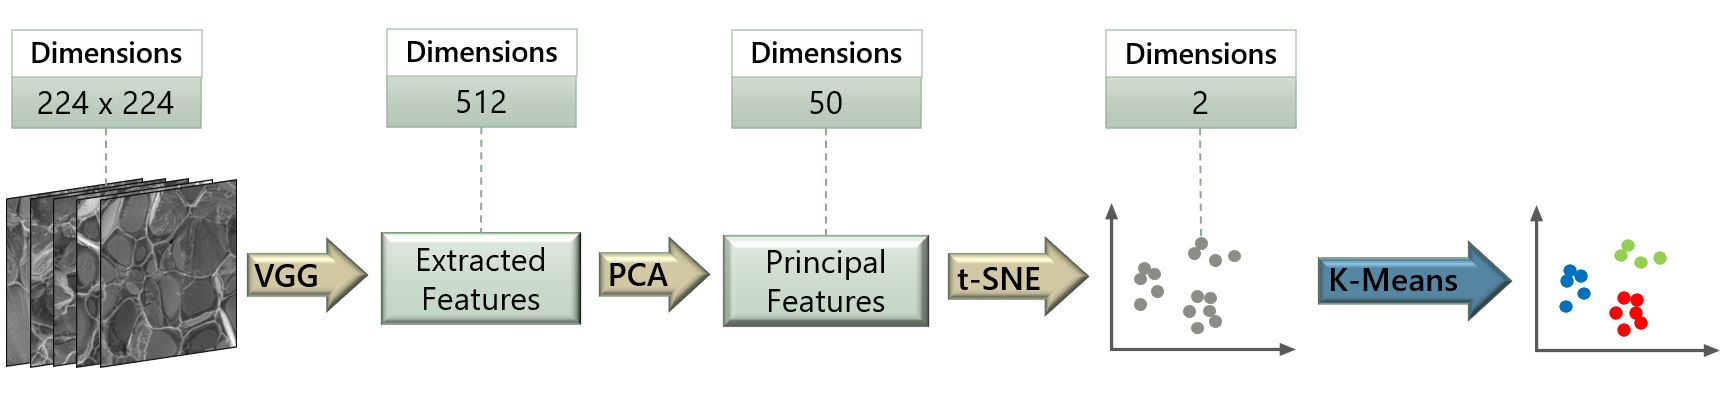
\includegraphics[width=\textwidth]{cluster_pipeline_2.jpg}
	\caption{Schematic flowchart of the clustering data pipeline.}
	\label{fig:cluster_pipe}
\end{figure}



The clustering algorithm is a 4-part data pipeline, where the dimensionality of the input data is reduced after each stage. A schematic flowchart of the algorithm is presented in Fig. \ref{fig:cluster_pipe} and the function of each stage is defined as follows:

\begin{itemize}
	\item \textbf{VGG16}: the VGG16 neural network architecture \citep{vgg}, where the final Fully-Connected layers are replaced by a Global Average Pooling (GAP) layer, is used to extract features from the input SEM fracture images. The network, using a set of pre-trained weights on the ImageNet dataset \citep{imagenet}, performs predictions on the SEM images. Each fracture image of the dataset is imported into the network and, after passing through all the consecutive layers, the last convolution layer outputs a sequence of 512 two-dimensional feature maps for each image. The GAP layer at the end of the network computes the mean value for each feature map and exports a feature vector in $\mathbb{R}^{512}$ for each input image. This modified network architecture enables the extraction of 512 features from each input image. Thus, a set of weights, although being trained on an extensive dataset of images that have no relevance to fracture images, when loaded to the modified VGG16 architecture allows the network to reduce the dimensionality of the input images from $224 \times 224$  to $512$ dimensions and extract meaningful information from the input data; the fracture images were resized to $224 \times 224$, before inserted into the VGG. 
	\item \textbf{PCA}: a Principal Component Analysis \citep{pca} on the feature vectors extracted by VGG allows the computation of the 50 principal components that maximize the total variance of the data. This linear-dimensionality reduction algorithm expresses each feature vector, which corresponds to a certain fracture image, with respect to 50 principal axes that maximize the total variance of the data. The algorithm enables the estimation of the "importance" of each principal component, by computing the eigenvalues of the covariance matrix of the set of feature vectors and furthermore the computation of the weight that each feature extracted by VGG has on each principal axis, by computing the eigenvectors of the covariance matrix. 
	\item \textbf{t-SNE}: this  algorithm \citep{tsne} performs a non-linear dimensionality reduction on the set of feature vectors in $\mathbb{R}^{50}$ that is exported by the PCA. It computes similarities between the data points in the 50-dimensional space and projects them onto the 2D space, according to these similarities. The final output of this stage is a 2D plot. By the end of this third part, the pipeline achieves to project the initial fracture images dataset onto data points on a 2D plot, in positions that enable clustering according to similarities of the fracture images.
	\item \textbf{k-Means}: the k-Means algorithm \citep{kmeans} groups the data points, exported by t-SNE into 5 clusters, according to their \textit{Euclidean} distances in the 2D space. As a result, k-Means assigns a label to each data point according to the cluster that it belongs.    
\end{itemize} 


This 4-part data pipeline is an unsupervised machine learning algorithm that groups any dataset into a predefined number of clusters, without requiring any training process; even the first part of the pipeline that is a neural network does not require additional training, since it implements the transfer learning technique. The computer code for this algorithm is developed in Python with the implementation of \textit{Keras} \citep{keras} and \textit{scikit-learn} \citep{sklearn} libraries; \textit{Keras} is used for building the VGG16 model and subsequently the inference operation of the first part of the pipeline, while the \textit{scikit-learn} functions are implemented for the other parts of the pipeline. The final output is a 2D scatter plot where the position of each data point is defined according to similarities on the high-dimensional space of the input dataset. The performance of this algorithm on the dataset of the WHA fracture image is evaluated in the next section. 

\subsection{Classification data pipeline}

The previous clustering pipeline can be extended into a classification algorithm, with the addition of a k-Nearest Neighbors (KNN) algorithm \citep{knn} at the end of the pipeline. The k-Nearest Neighbors is referred to as a \textit{minimal supervision} algorithm because the training process only involves saving the training data points and the corresponding labels. During the inference operation, the algorithm calculates the \textit{Euclidean} distances between each test data point and all the training data points, which enables the computation of \textit{k} nearest neighbors in the training dataset for each test data point. Finally, KNN assigns to each test data point the label that has the most representatives among the \textit{k} neighbors.

\begin{figure}[!h]
	\centering
	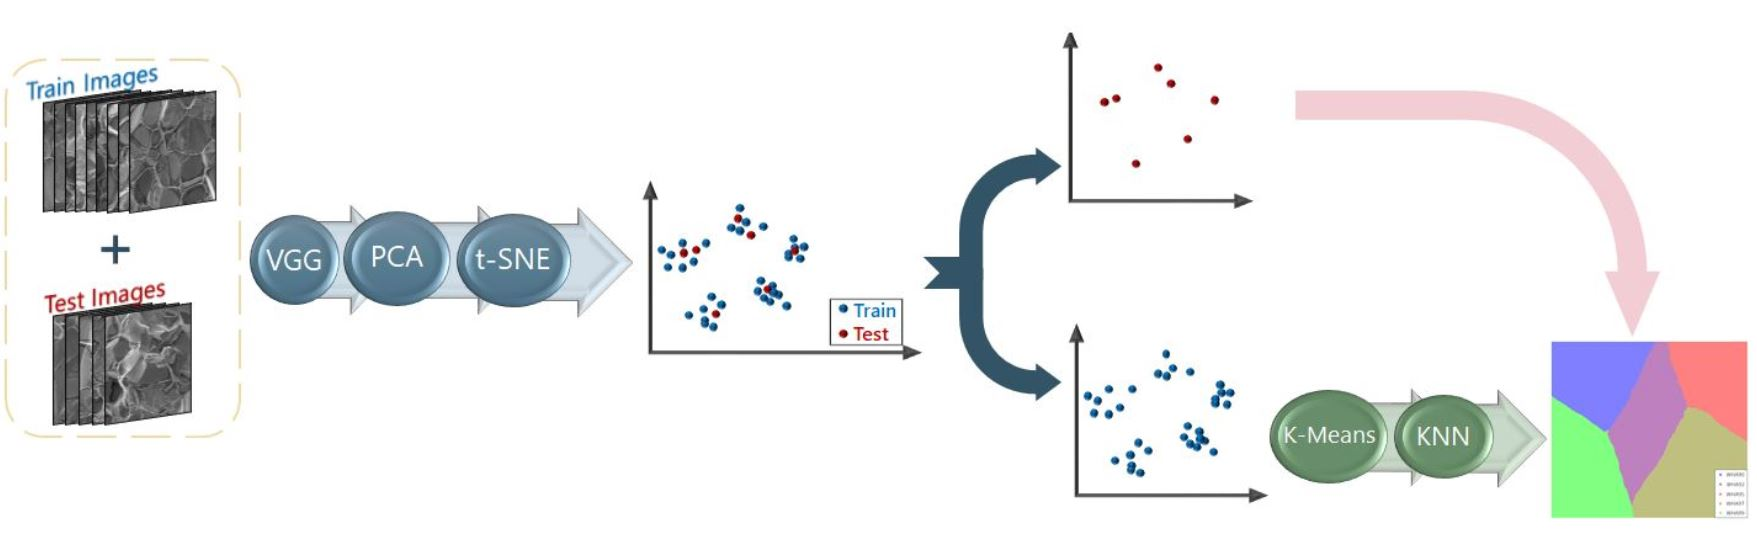
\includegraphics[width=\linewidth]{classification_pipeline_2.jpg}
	\caption{Schematic flowchart of the computation framework of the classification algorithm.}
	\label{fig:classif_pipe}
\end{figure}

The definition of a computational framework that combines the training and inference operations of the algorithm enables the classification of the fracture images according to the 5 tungsten composition labels.  A schematic flowchart of this computational framework is presented in Fig. \ref{fig:classif_pipe} and the outline of this computation process follows the next steps:

\begin{enumerate}
	\item Initially, 90\% of the WHA fracture images dataset is set as training images, while the rest 10\% is set as test images. 
	\item The entire dataset is imported into the \textbf{VGG} - \textbf{PCA} - \textbf{t-SNE} pipeline and the result is a 2D scatter plot. This plot is separated into a plot that contains only the training data points and another one with the test data points. 
	\item The training data points, projected onto the specific locations on the 2D plot by the \textbf{VGG} - \textbf{PCA} - \textbf{t-SNE} pipeline, are imported into another pipeline constructed by k-Means and KNN algorithms. 
	\item A mesh grid with dimensions large enough to accommodate every training and test data point is created and KNN enables the classification of every grid point into one of the 5 tungsten composition labels, using the training data points and their annotations. The result of this step is a colormap, where each area is assigned to a different tungsten composition label.
	\item The final step involves plotting the test data points, with the positions predicted by the \textbf{VGG} - \textbf{PCA} - \textbf{t-SNE} pipeline, onto the colormap. The label of the area that each test data point is placed defines the classification of the test point. 	
\end{enumerate}  


This computation process enables the classification of a fracture images test dataset according to pre-defined labels, when a training dataset with the corresponding annotations are provided. 


\section{Results and discussion}

\subsection{Clustering of fracture images}

The clustering data pipeline, presented in the previous section, is implemented on the dataset of WHA fracture images and the results are presented in this section. Different parameters for the intermediate algorithms of the pipeline have been investigated. More specifically, the PCA algorithm was tested with 50 or 100 principal components and t-SNE was implemented with Barnes-Hut approximation for the gradient computation \citep{barnes},  and it was tested for perplexity values in the range of (5, 50), learning rate in range (100, 1000) and the number of iterations was varied between 1000 to 10000 iterations. Finally, k-Means algorithm was tested with \textit{random} or \textit{k-means++} centroid initialization; \textit{kmeans++} is an initialization scheme for the cluster centroids, which has been implemented in scikit-learn according to \citet{kmeans2}.  

The combination of the parameter values that resulted into the best performance for this clustering pipeline is presented in Table \ref{table:clust}.  


\begin{table}[h]
	\centering
	\begin{tabular}[t]{ l  c } 
		\toprule
		Algorithm \hspace{1ex}  &  Parameters \\ \toprule
		PCA       \hspace{1ex}  &  Number of principal components = 50 \\
		t-SNE     \hspace{1ex}  &  Perplexity = 40, Learning rate = 200, Iterations = 3000 \\
		k-Means   \hspace{1ex}  &  Centroid initialization = \textit{k-means++} \\
		\bottomrule
	\end{tabular}
	\caption{Parameters of the clustering pipeline that enable the highest efficiency clustering of the WHA fracture images dataset.}
	\label{table:clust} 
\end{table} 

The dataset of 810 SEM images, obtained by fracture experiments on the WHA samples with different tungsten composition, is imported to the clustering data pipeline and the resulted 2D scatter plot is shown in Fig. \ref{fig:cluster_result}.


\begin{figure}[!h]
	\centering
	\fbox{\includegraphics[width=0.6\textwidth]{cluster_result.jpg}}
	\caption{Clustering results on the WHA fracture images dataset.}
	\label{fig:cluster_result}
\end{figure}
  
The initial qualitative assessment of the result shows that the algorithm succeeds in creating three distinct clusters (green, blue and red data points in the plot), while k-Means manages to separate the main cluster in the middle by assigning different labels to the data points. Subsequently, in order to quantify the performance of the algorithm the data points are plotted with their ground truth labels (Fig. \ref{fig:cluster_result_gt}). 

\begin{figure}[!h]
	\centering
	\fbox{\includegraphics[width=0.6\textwidth]{cluster_result_gt.png}}
	\caption{Ground truth of the clustering results on the WHA fracture images dataset.}
	\label{fig:cluster_result_gt}
\end{figure}

The ground truth plot shows that the algorithm fails to cluster correctly the data points that belong to the first SEM fracture image of the sample with 90wt\% tungsten composition; for each tungsten composition sample two SEM images were obtained and then cropped before added to the dataset, as it was explained in the beginning of the previous section. The erroneous predictions are marked (see crossed data points in Fig. \ref{fig:cluster_result_errors}) and the accuracy of the algorithm is computed to 81.2\%.


\begin{figure}[!h]
	\centering
	\fbox{\includegraphics[width=0.6\textwidth]{cluster_result_errors.png}}
	\caption{Clustering results with errors in predictions marked by crossed data points.}
	\label{fig:cluster_result_errors}
\end{figure}

Additionally, the confusion matrix presented in Fig. \ref{fig:confusion_mat} verifies that the main source of clustering errors is the data points that originate from the first SEM fracture image of the  sample with 90wt\% tungsten composition.
 
\begin{figure}[!h]
	\centering
	\includegraphics[width=0.5\textwidth]{confusion_mat.png}
	\caption{Confusion matrix of the clustering results shows that the first SEM image from the sample with 90wt\% tungsten composition is the main source of clustering errors.}
	\label{fig:confusion_mat}
\end{figure} 

In numerous tests on the same dataset, the accuracy of the algorithm in clustering the WHA fracture images was never exhibited a value below 73\%.


\begin{figure}[!h]
	\centering
	\fbox{\includegraphics[width=0.6\textwidth]{cluster_result_errors_without_A102.png}}
	\caption{Clustering results, after removing the data points of the first SEM image of the sample with 90wt\% tungsten composition, with errors in predictions marked by crossed data points.}
	\label{fig:cluster_result_errors2}
\end{figure}


Subsequently, the dataset images that belong to the first SEM image of the sample with tungsten composition of 90wt\% are removed and the accuracy of the algorithm in clustering the remaining dataset images  is computed. In Fig. \ref{fig:cluster_result_errors2} the clustering result is presented, with the errors being crossed as before. The improvement is significant and the confusion matrix (Fig. \ref{fig:confusion_mat2}) shows a uniform distribution of errors. Finally, the accuracy is raised to 91\%, after removing the data from this particular SEM image that the algorithm failed to cluster correctly. 

\begin{figure}[!h]
	\centering
	\includegraphics[width=0.5\textwidth]{confusion_mat_without_A102.png}
	\caption{Confusion matrix of the clustering results, after removing the data points of the first SEM image of the sample with 90wt\% tungsten composition.}
	\label{fig:confusion_mat2}
\end{figure} 

The visual differences between the two SEM images of the sample with 90wt\% tungsten composition are obvious, as it can be seen in Fig. \ref{fig:se}, and this explains the failure of the algorithm in grouping the data points that originated from these two images in the same cluster. This observation initiated the inquiry of the internal functions that enable the clustering operation of the algorithm. 

The question that arises is:

\begin{itemize}
	\item[--] \textit{Which features of the fracture images "attract the attention" of the neural network and from these extracted features which weigh more in the final result of the dimensionality reduction algorithms?}
\end{itemize}
     
The answer to this question is the subject of the last part of this section, which focuses on the visualization of the activation maps of the neural network and the interpretation of the functionality of the clustering algorithm that enables its efficacy.


\begin{figure}[!h]
	\centering
	\begin{subfigure}[b]{0.49\textwidth}
		\centering
		\includegraphics[width=\textwidth]{A_102.png}
		\caption{A102: first SEM image of the 90wt\% tungsten composition sample.}
		\label{fig:A_102}
	\end{subfigure}
	\begin{subfigure}[b]{0.49\textwidth}
		\centering
		\includegraphics[width=\textwidth]{A_103.png}
		\caption{A103: second SEM image of the 90wt\% tungsten composition sample.}
		\label{fig:A_103}
	\end{subfigure}
	\caption{The two SEM images obtained after scanning the sample with the 90wt\% tungsten composition. Note that both images are taking under the same magnification and field of view}
	\label{fig:se}
\end{figure}

  
 
\subsection{Fracture images classification}

The WHA fracture images dataset, without including the dataset images from the A102 SEM image (in Fig. \ref{fig:A_102}), is imported into the classification algorithm. 675 images of this dataset are assigned to training and the rest 54 are considered as the test images. Following the computational framework for the classification of the dataset, the algorithm is plotting the data point that correspond to the test images onto a colormap that defines the labels for the different tungsten compositions. For the k-Nearest Neighbors algorithm in the classification data pipeline, the number of nearest neighbors is set to $k=15$ and uniform weight distribution is used.

\begin{figure}[!h]
	\centering
	\begin{subfigure}[b]{0.49\textwidth}
		\centering
		\includegraphics[width=\textwidth]{classification.png}
		\caption{The result of the classification for the WHA dataset.}
		\label{fig:classification}
	\end{subfigure}
	\begin{subfigure}[b]{0.49\textwidth}
		\centering
		\includegraphics[width=\textwidth]{classification_gt.png}
		\caption{The ground truth labels of the classification result.}
		\label{fig:classification_gt}
	\end{subfigure}
	\caption{Classification results and ground truth annotations, with classification errors inside the red circles.}
\end{figure}

The result of this classification process is presented in Fig. \ref{fig:classification}. The position that each test data point on the colormap, which is computed by the classification data pipeline, defines the label that is assigned to the data point. Knowing the ground truth annotations for the test data points allows the evaluation of the classification errors (data points inside the red circles in Fig. \ref{fig:classification_gt}) and enables the computation of the classification accuracy. The accuracy of the classification predictions is computed to 93\%, while in numerous tests performed on the same dataset the lowest accuracy was 85\%.  
 
   



\subsection{Comparison with Haralick texture descriptors method}

The evaluation of the clustering and classification results shows that the two algorithms presented here exhibit very high accuracy when performing on a dataset of fracture images with very similar structural and morphological characteristics. 

In order to have a reference and better understanding of the algorithm efficiency, the WHA dataset is imported into an algorithm that extracts different texture descriptors and consequently enable image classification, following the method proposed by \citet{haralick}. The central component of this statistical methodology, which is commonly used for images classification tasks where texture is of importance (e.g. fractographs), is the Gray Level Cooccurrence Matrix (GLCM). The Haralick method defines 14 texture descriptors, which after being trained on a training dataset, enable classification on the fracture images of a test dataset. 

The performance of the Haralick texture descriptors algorithm on the WHA fracture images dataset is very poor, with classification accuracy of 21\%. Practically, this evaluation shows that the algorithm, which is based on a well-established method commonly used  for image classification, fails to classify the fracture images of the WHA dataset and reveals the complexity of the task at hand. Additionally, it shows the great potential of the Clustering and Classification algorithms that are presented in this paper and makes more evident the importance of their high efficiency performance.        


\subsection{Features visualization and Interpretability}

The objective of this section is to understand the internal functions that enable the clustering, and as an extension the classification, pipeline in performing with the reported high efficacy on the task at hand. More specifically, the study focuses on the visualization and consequently the interpretation of the features that the algorithm is identifying in the input fracture images and through this information aims to gain a better understanding on how these extracted features enable accurate predictions. 

Considering the architecture of the VGG16 network, the output of the last convolution layer is a set of 512 activation maps, with dimension of $7 \times 7$, for each input fracture image. This set is  denoted as: $\{\textbf{A}_k^c \; | \; k=1,2, ... M \text{ and } c=1,2, ... N\}$, where $N=810$ is the total number of images in the dataset and $M=512$ the number of activation maps. When this set of activation (or else feature) maps is inserted into the Global Average Pooling (GAP) layer, it exports a vector ($\vec{a}_c \in \mathbb{R}^{512}$) with the mean values of the extracted activation maps from each image. This set of feature vectors, $\{\vec{a}_c \; | \; c=1,2, ... N\}$, is imported into PCA. Initially, the PCA algorithm creates a data matrix $\textbf{X}$, with dimensions $N \times M$, by placing the feature vectors $\vec{a}_c$ in the rows of the matrix, and then computes the covariance matrix $\textbf{S}$, with dimensions $M \times M$, as follows: 

\begin{equation*}
\textbf{S} = \textbf{X}^T \cdot \textbf{X}
\end{equation*}

Finally, the computation of the eigenvalues ($\lambda_k$) and the eigenvectors ($\vec{u}_k$) of the covariance matrix are computed with the Singular Value Decomposition (SVD) method. 

The eigenvalues express the total variance of the linear combinations of the feature vectors ($\vec{a}_c$) with the computed eigenvectors ($\vec{u}_k$), which are called \textit{Principal Components} and their mathematical definition is:

\begin{equation*}
\vec{P}_k = \textbf{X} \cdot \vec{u}_k
\end{equation*}

This enables the representation of the 512-dimensional dataset of the feature vectors with respect to the $p=50$ principal components with the highest eigenvalues. Furthermore, the eigenvalues express the importance of each principal component on the reduced dimensionality representation and the eigenvectors that correspond to each principal components express the importance of each of the 512 extracted features by the VGG network on the specific component. Thus, selecting the first principal component it becomes possible to weigh its influence in the reduced dimensionality dataset, through the computation of the corresponding eigenvalue, and even assign a weight to each feature extracted by VGG on this specific component, by computing the 512 coefficients of the corresponding eigenvector. The coefficients of the corresponding eigenvector are the weights of the VGG extracted features.

The computation of the eigenvalues from the PCA algorithm of the clustering pipeline on the WHA dataset shows that the first principal component expresses 41.6\% of the information in the reduced dimensionality representation of the dataset. Note that the second and the third principal components express 16.5\% and 8.7\% of the information, respectively, while the influence of the rest of the principal components is even less significant.  

Following this analysis becomes apparent that for each input fracture image $c$ of the WHA dataset, the weighted, by the coefficients of the eigenvector of the first principal component, sum of all the activation maps exported by the final convolution layer will show the exact features of the input image that are utilized by the clustering algorithm in the process of grouping this image with the rest of the images in the WHA fracture images dataset. This conclusion is mathematically defined as follows:

\begin{equation*}
\textbf{A}_{heatmap}^c = \sum_{k=1}^{512} |w_k| \cdot \textbf{A}^c_k 
\end{equation*}  

where the set  $\{\textbf{A}^c_k \; | \;  k=1,2, ... 512 \text{ and } c=constant\}$ is the set of the activation maps for the specific input image and  $|w_k|$ are the absolute values of the coefficients of the eigenvector $\vec{u}$ that corresponds to the first principal component of the PCA:

\begin{equation*}
\vec{u} = \begin{bmatrix}  w_1 \\
						   w_2 \\
						  \cdot \\
						  \cdot \\
						  \cdot \\
						  w_{512}
		   \end{bmatrix}
\end{equation*}

The resulted activation heatmap $\textbf{A}_{heatmap}^c$ has dimensions of $7 \times 7$ and when resized to the original dimensions of the input image ($448 \times 448$ pixels) enables the localization of the features that the clustering algorithm is identifying in the specific image $c$ of the WHA dataset.

Implementing this computational framework in a python algorithm enables the visualization of the set of activation heatmaps: $\{\textbf{A}_{heatmap}^c \; | \; c=1,2, ... N\}$, computed for each fracture image of the WHA dataset. Fig. \ref{fig:activ_maps} presents some representative activation heatmaps from each group of tungsten composition, while the entire set of activation heatmaps, which counts 810 images, together with the corresponding WHA fracture images dataset are published in Materials Data Facility (MDF) with DOI: \url{https://doi.org/10.18126/aph0-olbz}. 


\begin{figure}[H]
	\centering
	\includegraphics[width=0.8\textwidth]{fmaps_bar_2.png}
	\caption{Activation heatmaps for a representative sub-set of the WHA fracture dataset.}
	\label{fig:activ_maps}
\end{figure} 


A careful examination of the activation heatmaps concludes that the algorithm is focusing on the ductile fracture of the alloy material, since it activates the areas between the tungsten grains that accommodate deep and clear dimples. This ductile behavior is  attributed to the fracture of nickel-Ferrous (NiFe) matrix and it can be hypothesized that the identification of the ductility of the fracture surface enables the algorithm to cluster the images according to the composition of nickel in the alloy material. Apparently, the algorithm does not focus on the tungsten's fracture and this very interesting observation can be justified by the fact that the fracture of tungsten can have different manifestations (intergranular or transgranular micro-fracture modes) in the alloy's fracture surface, which makes the identification more complex. This hypothesis provides a very reasonable interpretation of the internal operation of the clustering algorithm that enables the accurate clustering and elucidates the algorithm's efficacy in identifying the different fracture images. 

Although this analysis interprets the operation of the algorithm and the internal processes that enable the high efficiency clustering, it does not provide an explanation on the fact that the algorithm fails to group the two SEM fracture images from the sample with 90wt\% tungsten composition. In order to address this issue, the activation heatmaps from the fracture images, cropped from the two original SEM images obtained by scanning this particular sample (see Fig. \ref{fig:se}), are used to reconstruct the activation heatmaps that correspond to these two initial SEM images. 

In Fig. \ref{fig:A_activ} the activation heatmaps are shown. It is evident from these images that the algorithm has activated fewer areas in the activation heatmap of the image A102 compared to the activated areas in the heatmap of the A103 image. Following the previous analysis, the algorithm considers that the surface area of image A102 presents less ductility than the surface in the image A103. It is clear that a WHA sample produced with a specific tungsten composition - in this case 90wt\% - does not provide a fracture surface with uniform tungsten composition and it can be perfectly reasonable that the different areas that have been scanned by the SEM contain different ratios of tungsten and nickel, hence accommodating different amount of areas with ductile fracture. Thus, the activation heatmaps in Fig. \ref{fig:A_activ} can provide an interpretation of the failure of the algorithm in grouping the data from these two SEM images.   

\begin{figure}[!h]
	\centering
	\begin{subfigure}[b]{0.49\textwidth}
		\centering
		\includegraphics[width=\textwidth]{A_102_AM.png}
		\caption{Activation heatmap corresponding to A102.}
		\label{fig:A_102_am}
	\end{subfigure}
	\begin{subfigure}[b]{0.49\textwidth}
		\centering
		\includegraphics[width=\textwidth]{A_103_AM.png}
		\caption{Activation heatmap corresponding to A103.}
		\label{fig:A_103_am}
	\end{subfigure}
	\caption{Activation heatmaps that correspond to the two SEM images obtained after scanning the sample with the 90wt\% tungsten composition.}
	\label{fig:A_activ}
\end{figure}


Finally, the confusion matrix in Fig. \ref{fig:confusion_mat} shows that the data points that belong to the images cropped from the A102 SEM image are mainly clustered together with the data points obtained by the sample with 97wt\% tungsten composition and secondarily with the data points from the 92wt\% tungsten composition sample. Fig. \ref{fig:ABD_activ} presents the activation heatmaps of the SEM images whose data points are grouped together by the clustering algorithm. The similarities between the activation heatmaps of the A102 SEM image and the maps from the other two samples are significant and certainly more pronounced than the similarities between the A102 and A103 SEM images, which are obtained from the same sample.   


\begin{figure}[!h]
	\centering
	\begin{subfigure}[b]{0.45\textwidth}
		\centering
		\includegraphics[width=\textwidth]{A_102_AM.png}
		\caption{A102}
	\end{subfigure}
	\begin{subfigure}[b]{0.45\textwidth}
		\centering
		\includegraphics[width=\textwidth]{B_201_AM.png}
		\caption{92wt\%}
	\end{subfigure}
	\begin{subfigure}[b]{0.45\textwidth}
		\centering
		\includegraphics[width=\textwidth]{D_402_AM.png}
		\caption{97wt\% }
	\end{subfigure}
	\caption{Activation heatmaps that correspond to samples with (a) 90wt\% (b) 92wt\% (c) 97wt\% tungsten composition.}
	\label{fig:ABD_activ}
\end{figure}


Undoubtedly, a more systematic study of this clustering algorithm with different fracture datasets is required to prove or disprove the assumptions that are made in this interpretation of the algorithm's internal operation analysis. This paper encourages further investigation and the authors are convinced that a profound understanding of the functionality of the recently introduced Machine Learning algorithms can open up new possibilities with novel efficient characterization tools that optimize current methods in Fracture Mechanics.          
  
%\begin{figure}[!h]
%	\centering
%	\begin{tabular}[t]{c}
%		\includegraphics[width = 0.85\linewidth]{WHA90_fmaps.jpg}  \\ 
%		\includegraphics[width = 0.85\linewidth]{WHA92_fmaps.jpg}  \\ 
%		\includegraphics[width = 0.85\linewidth]{WHA92_fmaps.jpg}  \\ 
%		\includegraphics[width = 0.85\linewidth]{WHA92_fmaps.jpg}  \\ 
%		\includegraphics[width = 0.85\linewidth]{WHA92_fmaps.jpg} 
%	\end{tabular}
%	\caption{Activation heatmaps for a representative sub-set of the WHA fracture dataset.}
%	\label{fig:activ_maps}
%\end{figure}
  

\section*{Summary}
\label{conclusions_label}

This paper evaluates the performance of an \textit{Unsupervised Machine Learning} data pipeline in the clustering and classification of the SEM fracture images obtained from WHA samples with different tungsten compositions. The algorithm achieves to cluster the fracture images of this dataset according to their tungsten composition with accuracy that reaches to 81.2\%. Additionally, the data points that are erroneously clustered belong mainly to a certain SEM image and when they are removed from the dataset the accuracy of the algorithm raises to 91\%. 

Subsequently, by adding a \textit{minimally supervised} Machine Learning algorithm at the end of the clustering pipeline and defining a new computational framework, the classification of the fracture images according the tungsten composition of the sample that they belong is enabled. The classification accuracy is computed to 93\%, while the Haralick texture descriptors fail to classify this fracture images dataset, since they achieve accuracy of 21\%. 

Finally, in an attempt to interpret the functionality of the clustering algorithm, this research work introduces a method that enables the visualization of the features in the input fracture images that are activated by the algorithm and enable the identification and clustering of the images according to the tungsten composition. More specifically, a set of activation heatmaps - one for each input fracture image - is computed to enable the visualization of the exact locations in each input fracture image that are activated by the algorithm and consequently are used to enable the accurate clustering of the dataset. The interpretation of these activation heatmaps shows that the algorithm is using the ductile micro-fracture modes (dimples), which are the product of the ductile fracture of the Nickel-Ferrous matrix, in order to group the WHA dataset according to the tungsten composition. This estimation of ductility of the fracture surfaces is correlated to both the percentage of the NiFe presence in the alloy as well as to the relative amount of matrix failure exhibited by the specimen and this creates a criterion for the clustering process.  One can speculate, that since different loading scenarios (eg. loading rate, triaxiality etc.) will result in different crack paths and will affect the relative amount of ductile vs brittle fracture indicators in the surface, a similar pipeline could be used to classify specimens following the conditions at which they failed. This hypothesis will be tested in a future work.   
 

\section*{Data availability} The  dataset used for this study and the corresponding Activation Maps are published in Materials Data Facility (MDF) with DOI: \url{https://doi.org/10.18126/aph0-olbz}. The source code is available at \url{https://github.com/SteliosTsop/WHA_Clustering_Classification_Visualization}.  

\section*{Acknowledgments}
	The financial support provided by the Pazy foundation young researchers award Grant $\#$ 1176  and the European Union's Horizon2020 Programme (Excellent Science, Marie-Sklodowska-Curie Actions) under REA grant agreement $675602$ (Project OUTCOME), is gratefully acknowledged. 




\clearpage

\bibliography{References}
\bibliographystyle{elsarticle-harv}





\end{document}
